%! Author = Renatus Madrigal
%! Date = 3/6/2025

% Preamble
\documentclass[11pt]{article}

% Packages
\usepackage[
    left=1in,
    right=1in,
    top=1in,
    bottom=1in
]{geometry}
\usepackage{amsmath}
\usepackage{amsfonts}
\usepackage{amssymb}
\usepackage[ruled,vlined]{algorithm2e}
\usepackage{listings}
\usepackage{color}
\usepackage{tikz}
\usepackage{hyperref}

\usetikzlibrary{arrows.meta, positioning, shapes.geometric}

\definecolor{codegreen}{rgb}{0,0.6,0}
\definecolor{codegray}{rgb}{0.5,0.5,0.5}
\definecolor{codepurple}{rgb}{0.58,0,0.82}
\definecolor{backcolour}{rgb}{0.95,0.95,0.92}

\lstset{
    frame=tb,
    language=C++,
    basicstyle={\small\ttfamily},
    backgroundcolor=\color{backcolour},
    commentstyle=\color{codegreen}\itshape,
    keywordstyle=\color{blue}\bfseries,
    numberstyle=\tiny\color{codegray}\ttfamily,
    stringstyle=\color{codepurple}\ttfamily,
    breakatwhitespace=false,
    breaklines=true,
    captionpos=b,
    keepspaces=true,
    numbers=left,
    numbersep=5pt,
    showspaces=false,
    showstringspaces=false,
    showtabs=false,
    tabsize=4
}

\newtheorem{definition}{Definition}
\newtheorem{property}{Property}

\title{A report on the Mandelbrot set}
\author{Renatus Madrigal}
\date{\today}

% Document
\begin{document}

    \maketitle


    \section{Abstract}\label{sec:abstract}
    % TODO: Write abstract


    \section{Introduction}\label{sec:introduction}

    The Mandelbrot set constitutes a fractal structure characterized by an elegant mathematical definition that belies
    its extraordinary complexity.
    This project aims to explore the Mandelbrot set and its properties, as well as to provide a visual representation of
    the set using C++.
    This report will detail the algorithms and optimizations used to generate the Mandelbrot set.


    \section{Background}\label{sec:background}

    \begin{definition}
        Let $f_c(z) = z^2 + c$, where $z, c \in \mathbb{C}$.
        Sequence $\{z_n\}$ is defined by $z_0 = 0$ and $z_{n+1} = f_c(z_n)$.
        The \textbf{Mandelbrot set} $M$ is defined as follows:
        \begin{equation}
            M = \{c \in \mathbb{C} : \lim_{n \to \infty} |z_n| < \infty\}\label{eq:mandelbrot_set_define}
        \end{equation}
    \end{definition}

    It can be proved\textsuperscript{\cite{branner1989mandelbrot}} that the Mandelbrot set has this property:

    \begin{property}
        \label{prop:bounded}
        $\forall n \in M,\ |z_n| \leq 2$
    \end{property}

    Thus, we can define the \textbf{layer function}:

    \begin{definition}
        Let $f_c(z) = z^2 + c$.
        The \textbf{layer function} $L_c(n)$ is defined as follows:
        \begin{equation}
            L(c) = \min\{n : z_n > 2\}\label{eq:layer_function}
        \end{equation}
    \end{definition}

    This function measures the escape speed of the sequence $\{z_n\}$.
    With these definitions and properties, we can generate the image of the Mandelbrot set and explore its properties.


    \section{Algorithms}\label{sec:algorithms}

    To generate the Mandelbrot set, we use the \textbf{Escape Time Algorithm}.

    \begin{algorithm}[H]
        \SetAlgoLined
        \caption{Escape Time Algorithm}
        \label{alg:escape_time_algorithm}
        \KwData{Complex number $c$, maximum number of iterations $N$}
        \KwResult{Number of iterations $n$}
        z = 0\;
        \While{$|z| \leq 2$ and $n < N$}{
            $z \leftarrow z^2 + c$\;
            $n \leftarrow n + 1$\;
        }
        \Return $n$\;
    \end{algorithm}

    The iteration threshold $N$ is conventionally configured at $N = 1000$
    , which establishes a balance between computational efficiency and visual fidelity.
    Our implementation employs this parameterization scheme for fractal generation.

    To enhance the structural analysis, we introduce a boundary detection methodology based on the gradient field of the
    layer function.
    This approach enables the reconstruction of high-fidelity visualizations preserving the set's topological features.
    Specifically, we use the Sobel edge detection operator to compute the discrete gradient approximation

    A Sobel operator is defined as follows:

    \begin{equation}
        \label{eq:sobel_operator}
        G_x = \begin{bmatrix}
                  -1 & 0 & 1 \\
                  -2 & 0 & 2 \\
                  -1 & 0 & 1
        \end{bmatrix}
        \quad
        G_y = \begin{bmatrix}
                  -1 & -2 & -1 \\
                  0  & 0  & 0  \\
                  1  & 2  & 1
        \end{bmatrix}
    \end{equation}

    Then, the gradient magnitude is computed as follows:

    \begin{equation}
        \label{eq:gradient_magnitude}
        \parallel \nabla L \parallel \ = \sqrt{(G_x * L)^2 + (G_y * L)^2}
    \end{equation}

    However, in practice, we approximate the gradient magnitude using the absolute value of the gradient components, and
    we take the arithmetic mean of the two components.
    This simplification allows for a more computationally efficient.

    Then, we set \textit{GradientThreshold}
    to 0.5, and pick out the pixels with gradient magnitude higher than the threshold.
    These pixels are likely to be on the edge of the Mandelbrot set, so we can automatically detect the boundary of the
    set.

    Here is the implementation:

    \begin{lstlisting}[label={lst:detect_high_gradient}, gobble=8]
        cv::Mat detectHighGradient(const cv::Mat &matrix) {
            constexpr static double GRADIENT_THRESHOLD = 0.5;

            cv::Mat normalized;
            cv::normalize(matrix, normalized, 0, 255, cv::NORM_MINMAX, CV_8UC1);

            cv::Mat grad_x, grad_y;
            cv::Sobel(normalized, grad_x, CV_32F, 1, 0);
            cv::Sobel(normalized, grad_y, CV_32F, 0, 1);

            cv::Mat abs_grad_x, abs_grad_y, grad_mag;
            cv::convertScaleAbs(grad_x, abs_grad_x);
            cv::convertScaleAbs(grad_y, abs_grad_y);
            cv::addWeighted(abs_grad_x, 0.5, abs_grad_y, 0.5, 0, grad_mag);

            double min_val, max_val;
            cv::minMaxLoc(grad_mag, &min_val, &max_val);
            double threshold = min_val + (max_val - min_val) * GRADIENT_THRESHOLD;

            cv::Mat mask = grad_mag;
            cv::threshold(grad_mag, mask, threshold, 255, cv::THRESH_BINARY);
            return mask;
        }
    \end{lstlisting}

    With the mask, we can detect the area with high gradient magnitude, which is likely to be the fractal boundary.
    In detail, we split the matrix with several blocks, and for each block, we calculate the total number of high
    gradient pixels.
    Then, we can determine the block with the most high gradient pixels, and we can zoom in on this area to get a more
    detailed image of the boundary.
    Here is the pseudocode:


    \begin{algorithm}[H]
        \SetAlgoLined
        \caption{Detect Boundary}
        \label{alg:detect_boundary}
        \KwData{Escape time matrix $matrix$, block rows and columns count $n$}
        \KwResult{Boundary area}
        $mask \leftarrow detectHighGradient(matrix)$\;
        $maxHighGradientPixels \leftarrow 0$\;
        $maxBlock \leftarrow null$\;
        Split matrix into $n \times n$ blocks\;
        \For{each block}{
            Count the number of high gradient pixels\;
            \If{high gradient pixels > maxHighGradientPixels}{
                $maxHighGradientPixels \leftarrow high gradient pixels$\;
                $maxBlock \leftarrow block$\;
            }
        }
        \Return maxBlock\;
    \end{algorithm}

    We pick out the maximum block and set its center as the new center of the image.
    Then, we zoom in on this area to get a more detailed image of the boundary.
    To implement this, we need to adjust the scale of the image and the center of the image.
    OpenCV provides several functions to generate the scale matrix, and we can use the \textit{warpAffine}
    function to adjust the image.
    These code are in \href{https://github.com/AI1379/MandelbrotSet/blob/master/src/VideoGenerator.h}
    {\texttt{src/VideoGenerator.h}}.


    \section{Optimizations}\label{sec:optimizations}

    To optimize the efficiency and precision of the Mandelbrot set generation, we introduce several optimizations.

    \subsection{Parallelism}\label{subsec:parallelism}

    In CPU versions, we use OpenMP to parallelize the computation of layer functions on each pixel.
    Thanks to the integrated OpenMP support in modern compilers, we can implement parallelism with minimal code as
    follows:

    \begin{lstlisting}[gobble=8, label={lst:openmp_parallel_for}]
        #pragma omp parallel for
    \end{lstlisting}

    In GPU versions, we use CUDA to accelerate the computation of layer functions.
    We split the image into blocks and assign each block to a CUDA thread.
    Then, we can compute the layer function for each pixel in parallel.
    These code are in \href{https://github.com/AI1379/MandelbrotSet/blob/master/src/MandelbrotSetCuda.cu}
    {\texttt{src/MandelbrotSetCuda.cu}}

    \subsection{Asynchronous pipeline}\label{subsec:asynchronous-pipeline}

    In video generation, the asynchronous workflow is a bit more complex.
    Thus, we introduce \texttt{P2300 - std::execution}\textsuperscript{\cite{P2300Proposal}}
    to build the asynchronous pipeline.
    The P2300 proposal provides a high-level abstraction for asynchronous execution, which is a candidate for standard
    C++ asynchrony and likely to be included in the C++26.
    An implementation of the asynchronous pipeline is available in GitHub repository
    \texttt{NVIDIA/stdexec}\textsuperscript{\cite{stdexec}}.
    As for the video generation, we design this asynchronous pipeline:

    \vspace{0.5cm}

    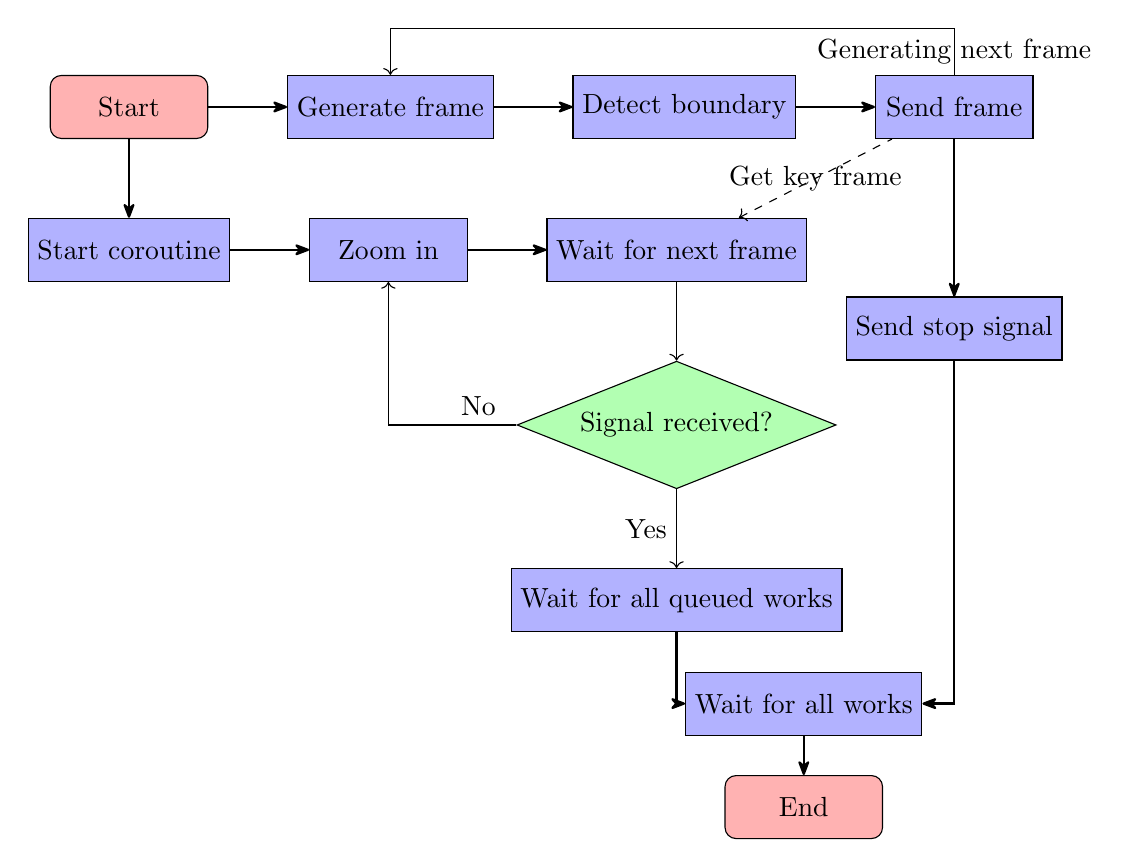
\begin{tikzpicture}[
        node distance=1.5cm,
        startstop/.style={
            rectangle,
            rounded corners,
            minimum width=2cm,
            minimum height=0.8cm,
            text centered,
            draw=black,
            fill=red!30
        },
        process/.style={
            rectangle,
            minimum width=2cm,
            minimum height=0.8cm,
            text centered,
            draw=black,
            fill=blue!30
        },
        decision/.style={
            diamond,
            aspect=2.5,
            minimum width=1cm,
            minimum height=1cm,
            text centered,
            draw=black,
            fill=green!30
        },
        arrow/.style={
            thick,
            ->,
            >=Stealth[round]
        }
    ]
        \node (start) [startstop] {Start};
        \node (coro) [process, below=1cm of start] {Start coroutine};
        \node (generate) [process, right=1cm of start] {Generate frame};
        \node (detect) [process, right=1cm of generate] {Detect boundary};
        \node (send) [process, right=1cm of detect] {Send frame};
        \node (stopsignal) [process, below=2cm of send] {Send stop signal};
        \node (zoom) [process, right=1cm of coro] {Zoom in};
        \node (wait) [process, right=1cm of zoom] {Wait for next frame};
        \node (waitsignal) [decision, below=1cm of wait] {Signal received?};
        \node (waitqueue) [process, below=1cm of waitsignal] {Wait for all queued works};
        \node (waitall) [process, below right=0.5cm and -2cm of waitqueue] {Wait for all works};
        \node (end) [startstop, below=0.5cm of waitall] {End};

        \draw [arrow] (start) -- (generate);
        \draw [arrow] (generate) -- (detect);
        \draw [arrow] (detect) -- (send);
        \draw [->] (send) -- node[midway] {Generating next frame} ++(0, 1) -| (generate);
        \draw [arrow] (start) -- (coro);
        \draw [arrow] (coro) -- (zoom);
        \draw [arrow] (zoom) -- (wait);
        \draw [<-, dashed] (wait) --node {Get key frame} (send);
        \draw [->] (wait) -- (waitsignal);
        \draw [->] (waitsignal) -- node[left] {Yes} (waitqueue);
        \draw [->] (waitsignal) -- node[above] {No} ++(-3, 0) -| (zoom);
        \draw [arrow] (send) -- (stopsignal);
        \draw [arrow] (waitqueue) |- (waitall);
        \draw [arrow] (stopsignal) |- (waitall);
        \draw [arrow] (waitall) -- (end);

    \end{tikzpicture}

    \vspace{0.5cm}

    With the facilities provided by the P2300 proposal, we can build a high-performance asynchronous pipeline for video
    generation.
    These code are in \href{https://github.com/AI1379/MandelbrotSet/blob/master/src/VideoGenerator.h}
    {\texttt{src/VideoGenerator.h}}.

    \subsection{Precision optimization}\label{subsec:precision-optimization}

    To optimize the precision of the Mandelbrot set, we introduce the \texttt{ExtendedDouble}
    type to store floating-point numbers with extended precision.
    It is implemented by combining an extra \texttt{int} to store the exponent and a \texttt{double}
    to store the mantissa.
    It is useful for high-precision computation, while its performance is comparable to the \texttt{double}
    and much faster than \texttt{mpfr\_t}.
    The implementation is in \href{https://github.com/AI1379/MandelbrotSet/blob/master/src/ExtendedDouble.cu}
    {\texttt{src/ExtendedDouble.cu}}

    \bibliography{references}
    \bibliographystyle{plain}
\end{document}